\subsection{Essential matrix}
Two methods are implemented for essential matrix estimation: the $8$-point algorithm and the $5$ point algorithm~\cite{nister2003efficient}~\cite{li2006five}~\cite{triggs2000routines}~\cite{nister2004efficient}. $8$ point algorithm is chosen since it is the most straight-forward method which gives only one solution, while $5$ point algorithm is the minimal solution for essential matrix estimation. It is easy to derive from $5$ point algorithm to other $6$ or $7$ point algorithms, although the $6$ or $7$ point algorithms were proposed earlier than $5$ point algorithms.

\subsubsection{$5$ point algorithm}
TODO a brief summary of $5$ point algorithm.

The most widely known $5$ point algorithms or implementations are listed here:
\begin{enumerate}
\item Nist\'er version in CVPR~\cite{nister2003efficient} and PAMI~\cite{nister2004efficient}. The PAMI version is favoured here since it is relatively simpler.
\item Gr\"obner basis version in~\cite{stewenius2006recent}. 
\item Polynomial Eigenvalue solution in~\cite{kukelovapolynomial}.
\end{enumerate}
Implementations:
\begin{itemize}
\item \url{https://github.com/prateekt/allyourposesrours}: a \textsc{Matlab} symbolic based implementation of Nist\'er five point algorithm.
\item archived at \url{https://web.archive.org/web/20170401223934/http://www.vis.uky.edu:80/~stewe/FIVEPOINT/}: a \textsc{Matlab} based Grobner Basis Method and a Nist\'er five point implementation.
\item \url{https://raw.githubusercontent.com/jianxiongxiao/SFMedu/master/peig5pt.m}: Polynomial Eigenvalue solution.
\item: two self developed implementations.
\end{itemize}
A performance and runtime evaluation can be seen from
\begin{figure}
\centering
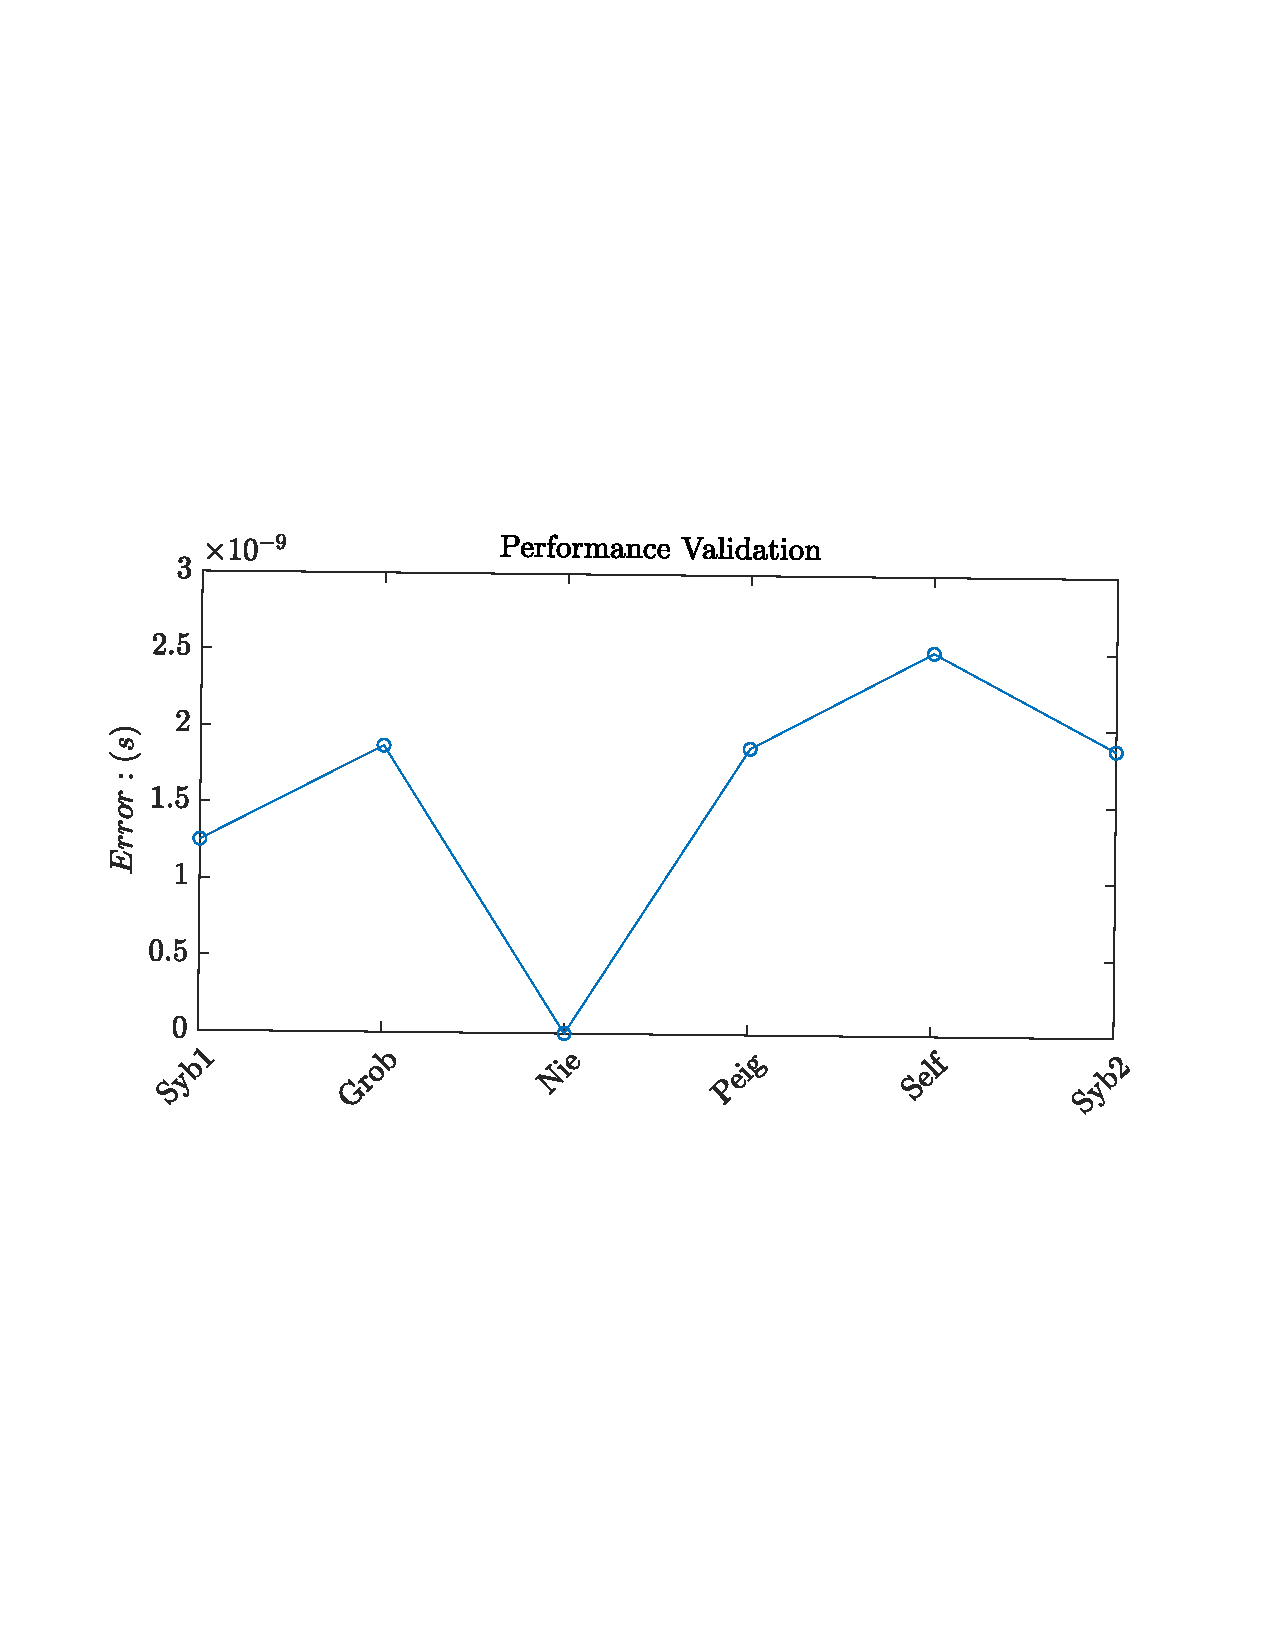
\includegraphics[width=0.45\textwidth]{hand_eye_files/vision/figures/five_point_perf}
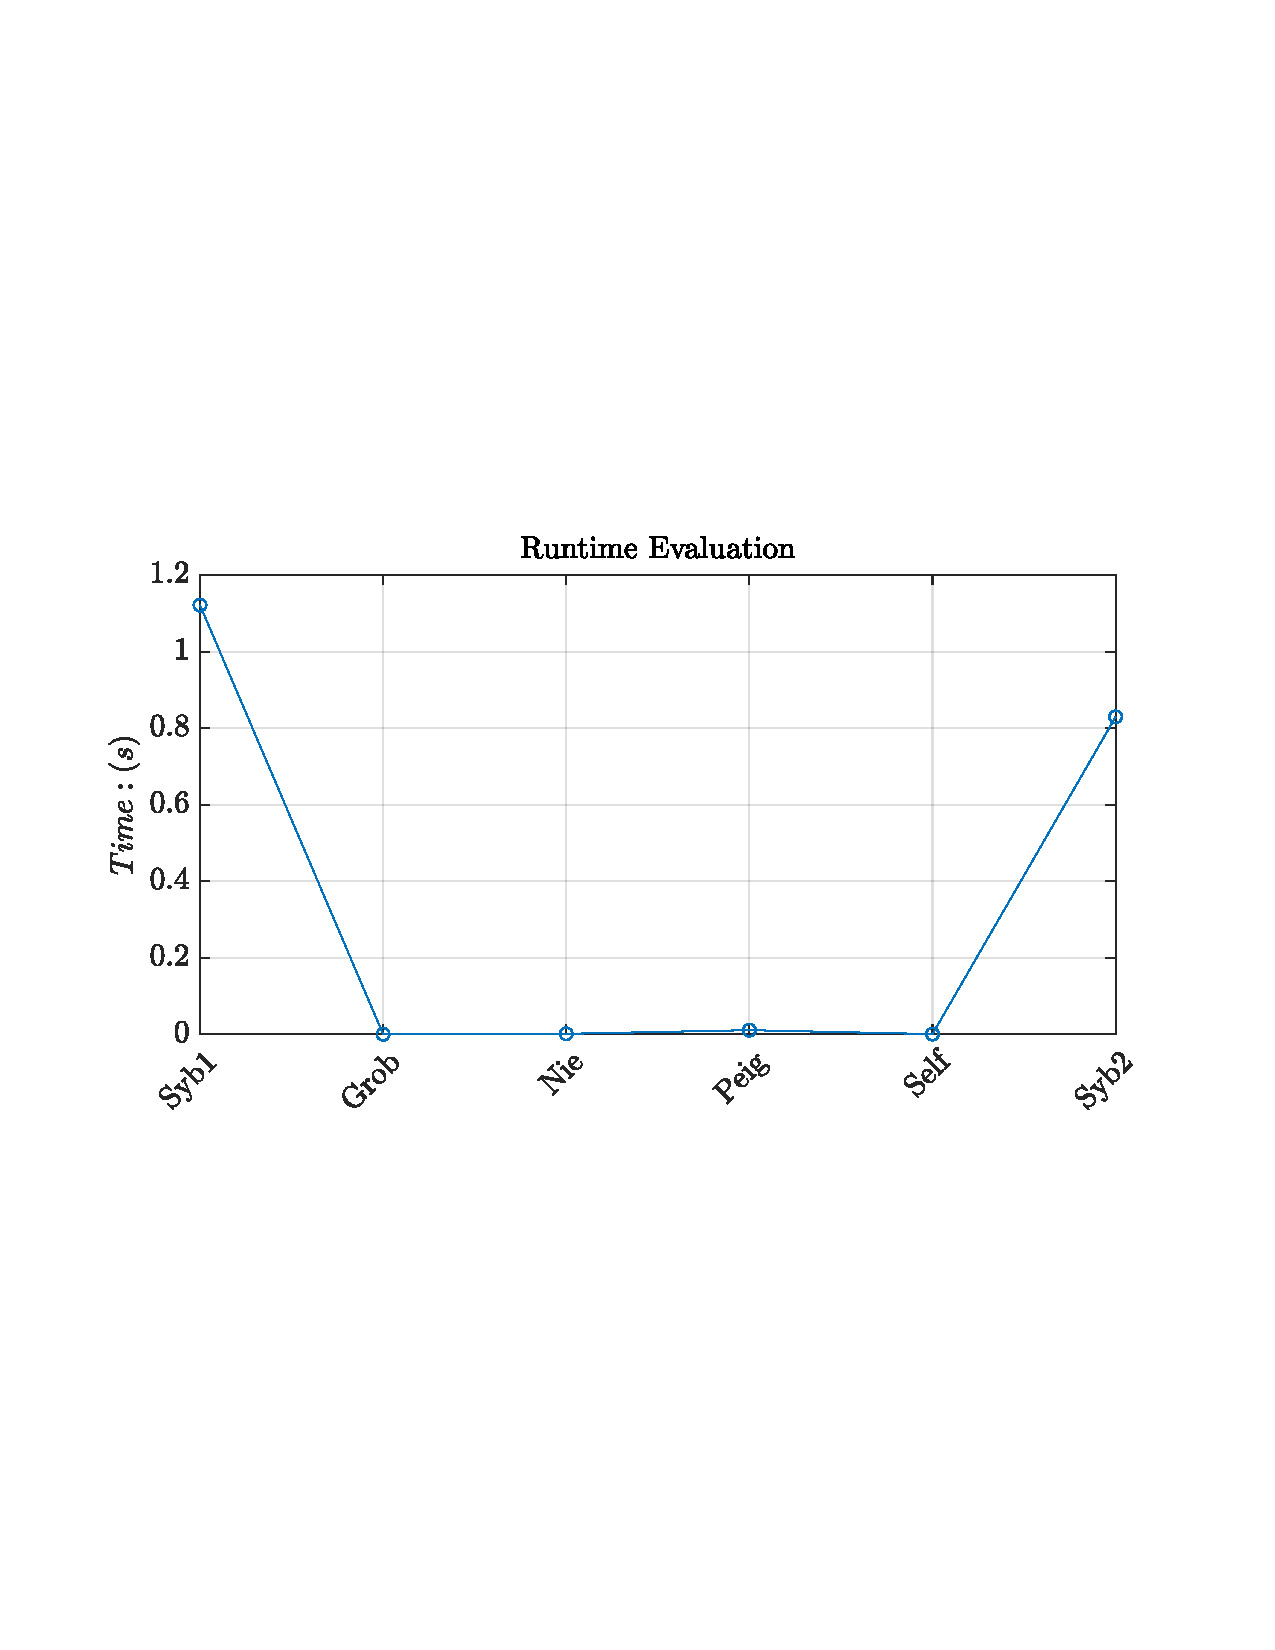
\includegraphics[width=0.45\textwidth]{hand_eye_files/vision/figures/five_point_time}
\label{fig:ess_com}
\end{figure}
\begin{table}[h!]
\centering
\caption{Details of runtime}
\begin{tabular}{c||c}
\hline
\textbf{Name} & \textbf{Time}: (s) \\
 Syb1 & $1.1213$ \\
 Grob & $0.0002$ \\
 Nie & $0.0015$ \\
 Peig & $0.0110$ \\
 Self & $0.0008$ \\
 Syb2 & $1.8294$ \\ 
 \hline
\end{tabular}
\label{tb:ess_com}
\end{table}
From this figure~\ref{fig:ess_com} and Table~\ref{tb:ess_com}, it can be seen Grob, Nie, Self are the three fastest methods. So they are chosen as the five point algorithm for future usage\footnote{$100$ Experiments are carried for evaluation.}.